\exer{[FIC-011-cor]}
\setcounter{numques}{0}~\\

\question{} 

La méthode read lit un caractère depuis la position courante, renvoie une chaine.

La méthode readline lit le reste de la ligne depuis la position courante, renvoie une chaine.

La méthode readlines lit toutes les lignes depuis la position courante, renvoie une liste de chaines.

\question{} 


Ce sont les caractères \og tabulation\fg{} et \og nouvelle ligne\fg{} .


\question{}

\begin{lstlisting}
def carac(nom_de_fichier):
    """Renvoie une liste contenant le nombre de caractères
       de chaque ligne de nom_de_fichier"""
    with open(nom_de_fichier,'r',encoding='utf8') as f:
        lignes = f.readlines()
    return [len(x.strip('\n').strip('\t')) for x in lignes]
\end{lstlisting}


\question{}

\begin{lstlisting}
def somme_carac(nom_de_fichier):
    """Renvoie la somme nombre de caractères
       du texte entier"""
    L=carac(nom_de_fichier)
    S=0
    for x in L:
        S+=x
    return S
\end{lstlisting}

\question{}
\begin{lstlisting}
def compte_carac(carac,nom_de_fichier):
    '''renvoie pour un caractère de l'alphabet son nombre d'occurence sans tenir compte de la casse contenu dans le fichier nom_de_fichier'''
    with open(nom_de_fichier,'r',encoding='utf8') as f:
        ligne='_'
        S=0
        while ligne!='':
            ligne = f.readline().lower()
            for c in ligne:
                if c==carac.lower():
                    S+=1
        return S
\end{lstlisting}

On peut utiliser une autre version plus courte.

\begin{lstlisting}
def compte_carac2(carac,nom_de_fichier):
    '''renvoie pour un caractère de l'alphabet son nombre d'occurence sans tenir compte de la casse contenu dans le fichier nom_de_fichier'''
    with open(nom_de_fichier,'r',encoding='utf8') as f:
        texte=f.read()
        return texte.lower().count(carac)
\end{lstlisting}


\question{}

\begin{lstlisting}
def stat_carac(nom_de_fichier):
    '''renvoie une liste de 26 éléments donnant le nombre d'occurrences de chaque lettre de l'alphabet contenu dans le texte nom_de_fichier sans tenir compte de la casse'''
    alphabet='abcdefghijklmnopqrstuvwxyz'
    occurrences=[]
    for car in alphabet:
        occurrences.append(compte_carac(car,nom_de_fichier))
    return occurrences
\end{lstlisting}


\question{}

Il faut importer ces modules et fonctions : 
\begin{lstlisting}
import matplotlib.pyplot as plt
from numpy import arange
\end{lstlisting}

\begin{minipage}{0.5\textwidth}
%\textbf{Méthode 1 : graphe}

\begin{lstlisting}
def tracer_occurrences(nom_de_fichier):
    ''' trace en fonction du numéro de la lettre dans l'alphabet son occurrence dans le fichier texttt{nom_de_fichier}'''
    y=stat_carac(nom_de_fichier)
    plt.clf()
    plt.plot(y,'ro')
    plt.xlabel("Numéro de la lettre dans l'alphabet")
    plt.ylabel('occurrences')
    plt.savefig('tp06_vosnoms_q10.png')
\end{lstlisting}

\end{minipage}
\begin{minipage}{0.5\textwidth}
\begin{center}
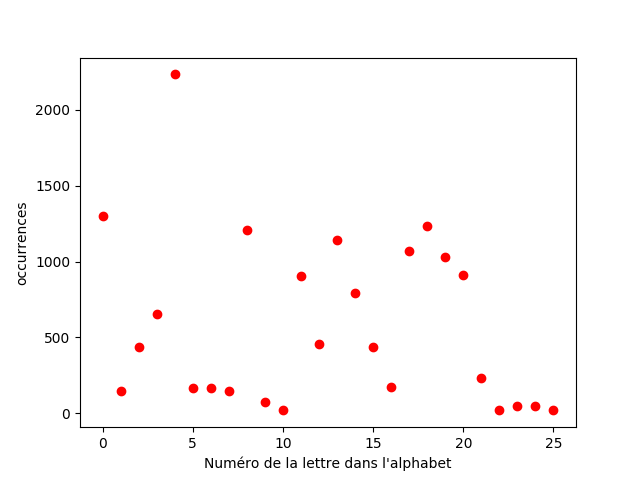
\includegraphics[width=0.9\textwidth]{tp06_vosnoms_q10.png}
\end{center}
\end{minipage}


%
%\begin{minipage}{0.5\textwidth}
%\textbf{Méthode 2 : histogramme}
%
%\begin{lstlisting}
%alphabet='abcdefghijklmnopqrstuvwxyz'
%alphabet_liste=len(alphabet)*[]
%for c in alphabet:
%    alphabet_liste.append(c)
%def trace_stat_carac_bis(nom_de_fichier):
%    y=stat_carac(nom_de_fichier)
%    plt.clf()
%    for i,yi in enumerate(y):
%        plt.plot([i,i],[0,yi],'r-',linewidth=5)
%    plt.ylabel('occurences')
%    plt.xticks(arange(26),tuple(alphabet_liste))
%    plt.savefig('histo_occurences.png')
%    plt.show()
%\end{lstlisting}
%
%\end{minipage}
%\begin{minipage}{0.5\textwidth}
%\begin{center}
%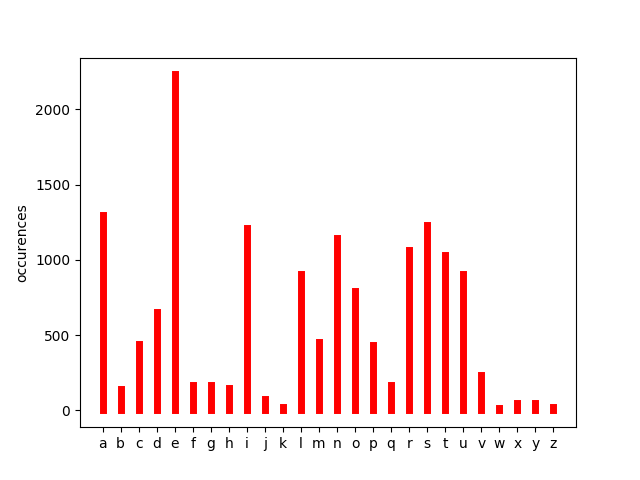
\includegraphics[width=0.9\textwidth]{histo_occurences.png}
%\end{center}
%\end{minipage}

\question{}

\begin{minipage}{0.5\textwidth}
%\textbf{Méthode 1 : graphe}

\begin{lstlisting}
def tracer_stat_occurrences(nom_de_fichier):
    y=stat_carac(nom_de_fichier)
    S=somme_carac(nom_de_fichier)
    plt.clf()
    for i,yi in enumerate(y):
        plt.plot([i,i],[0,100*yi/S],'r-',linewidth=5)
    plt.ylabel('Fréquences de caractères en %')
    plt.grid()
    plt.title(" Texte de Philippe Roth",fontsize=10)
    plt.xticks(arange(26),tuple(alphabet_liste))
    plt.savefig('tp06_vosnoms_q11.png')
\end{lstlisting}

\end{minipage}
\begin{minipage}{0.5\textwidth}
\begin{center}
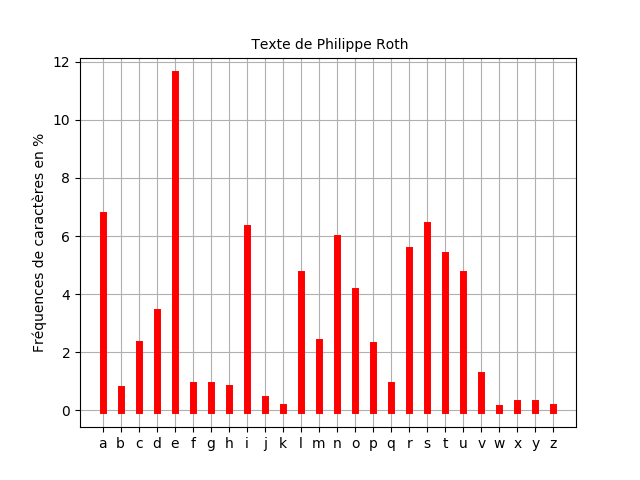
\includegraphics[width=0.9\textwidth]{tp06_vosnoms_q11.png}
\end{center}
\end{minipage}

\question{}



\begin{lstlisting}
def stat_carac_wikipedia(nom_de_fichier):
    '''à partir du fichier nom_du_fichier contenant les statistiques de fréquences de caractères renvoie une liste donnant en fonction de la position de la lettre dans l'alphabet sa fréquence en %.'''
    occurences=[]
    with open(nom_de_fichier,'r',encoding='utf8') as f:
        ligne = f.readline()
        while ligne!='':
            occurences.append(float(ligne.strip('\n').split(';')[1]))
            ligne = f.readline()
    return occurences
\end{lstlisting}


\question{} 

\begin{center}
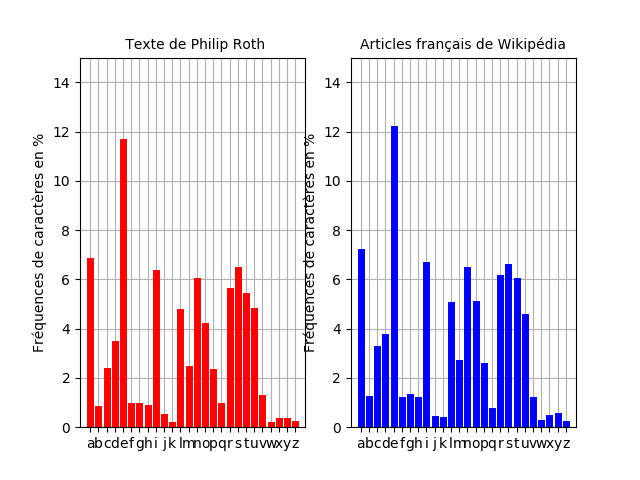
\includegraphics[width=0.9\textwidth]{histo_occurences_pourcent_comparaison.png}
\end{center}


